\chapter{Image Classification}
In order for algorithms such as EMC to work, the amount of heterogeneity within the diffraction data set has to be limited. Furthermore, each of the steps in the experiment introduces its own type of noise to the measured diffraction pattern. For example think of the debris clumping around small particles compared to the drop when sprayed with the GDVN, detector malfunctioning or saturation, or intensity fluctuations due to the random start of the SASE process. Often the results of the first two types of noise can not be tolerated by EMC, and image classification before the EMC step is necessary. Also fast feedback about the first type of noise is very useful to have during the experiment. So far a very robust sizing method has been developed, but more extended methods might come in useful. Several methods shown here can give rapid feedback on the heterogeneity of the particle.

%\section{Template-based classification}
%If your object has a known shape it could be possible to only select the diffraction patterns that are similar to a set of expected diffraction patterns from the object called templates. Paper III explores the possibility of template-based classification. In general this method is highly dependent on the choice of template, as well as the amount and type of variation present in your sample.

\section{Feature extraction}
A way of selecting diffraction patterns is by extracting general features from the diffraction pattern such as size, particle shape, amount of saturation, number of particles in the beam. Based on the relative values associated with the features individual patterns might be selected or discarded, or if these values are determined during an experiment, the experimental conditions might be rapidly adjusted. This section describes several feature extraction algorithms I have implemented.

\subsection{Size}
A common method to determine the size of an object is fitting the central speckle to the central speckle of simulated diffraction pattern from a sphere. This method has shown to be successful for particles that have an icosahedral to spherical shape \cite{Hantke2014,Daurer2017}. If the 3rd to the 5th minima are also present in the diffraction pattern, the average of these minima can also be used to determine the size of the object. This method can be especially useful in case the central speckle or first minimum cannot be evaluated reliably due to for example saturation effects. Figure \ref{fig:sizing} shows the relative reliability of using different minima to assess the size of an icosahedral object. These results rely on simulated diffraction patterns \cite{Hantke2016}.

\begin{figure}[h]
\centering
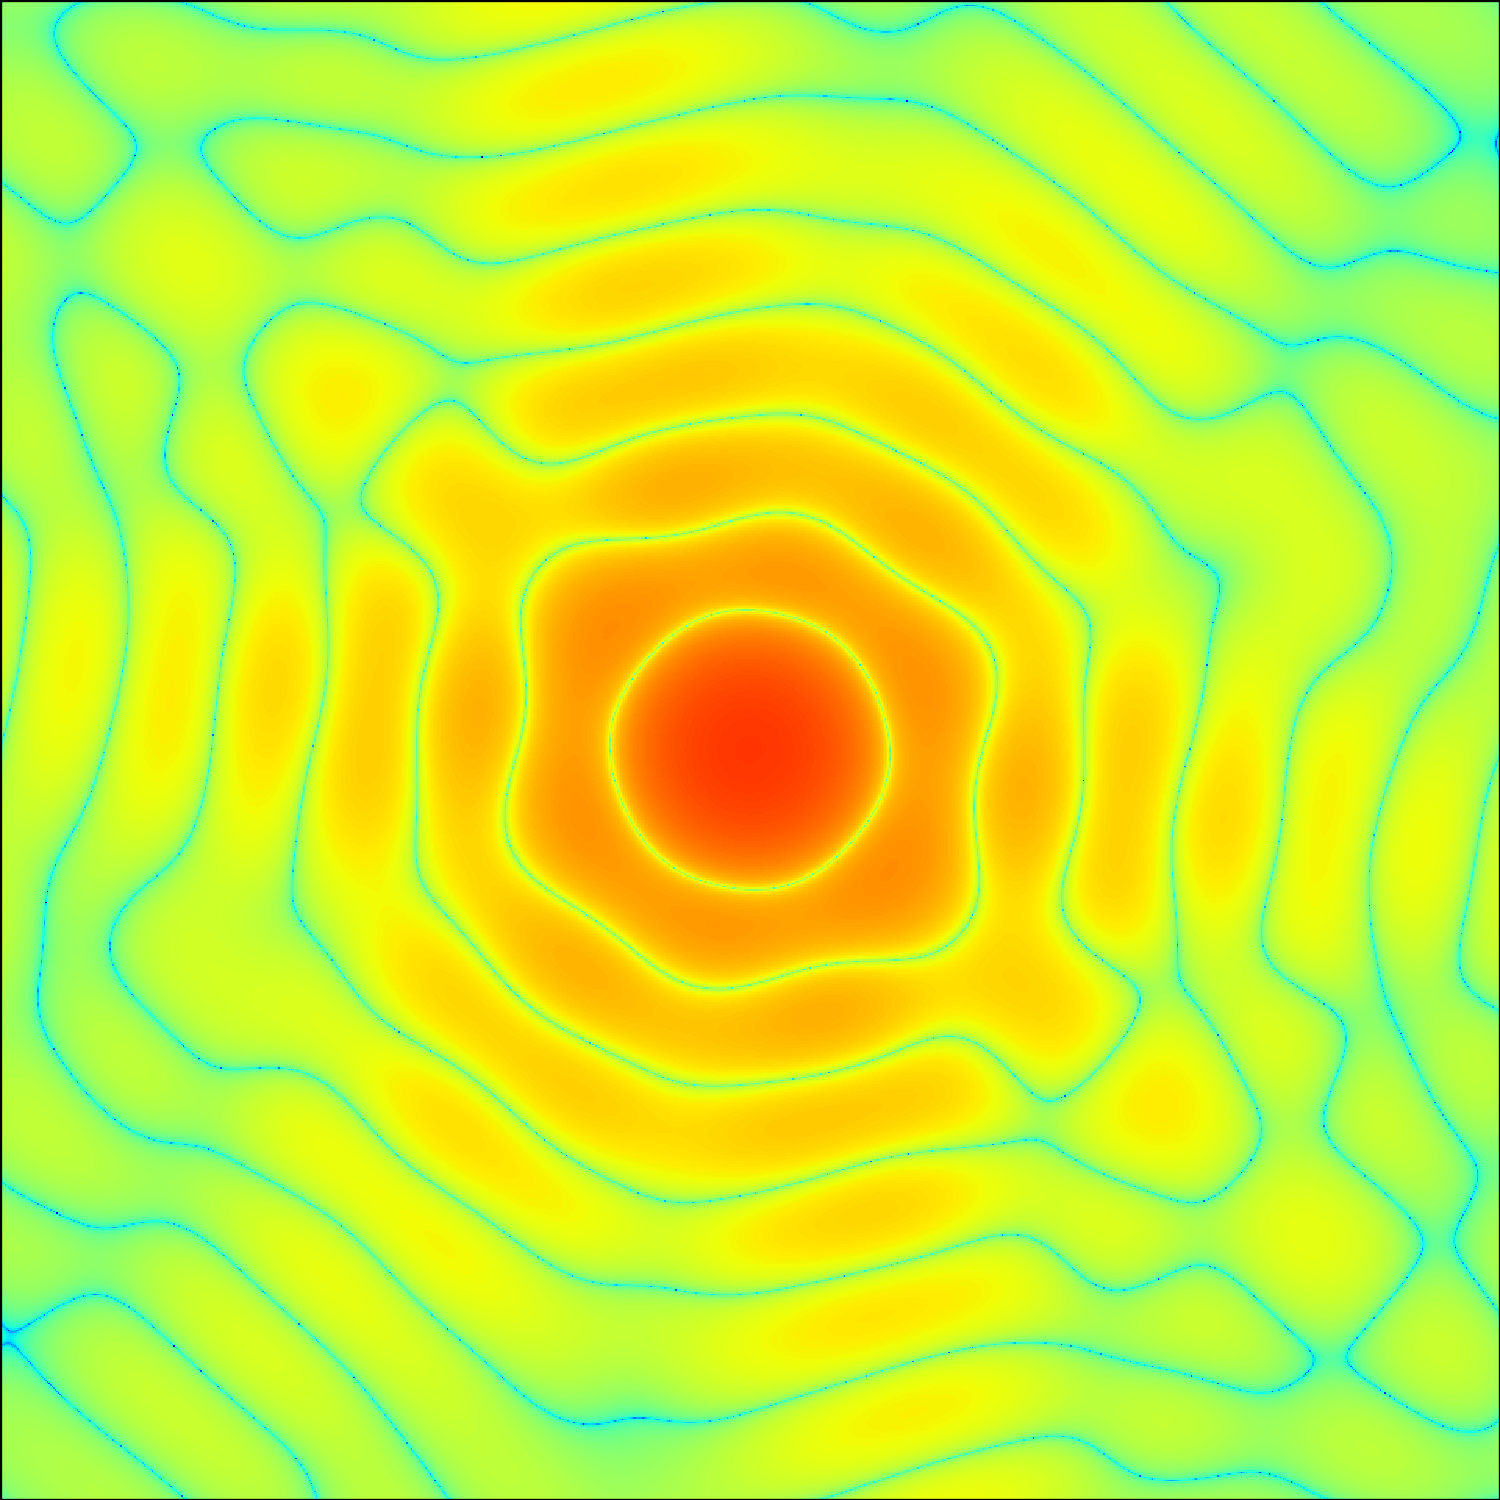
\includegraphics[width=42mm]{Chapter_08_ImageClassification_Simulated_Icosahedron.png}
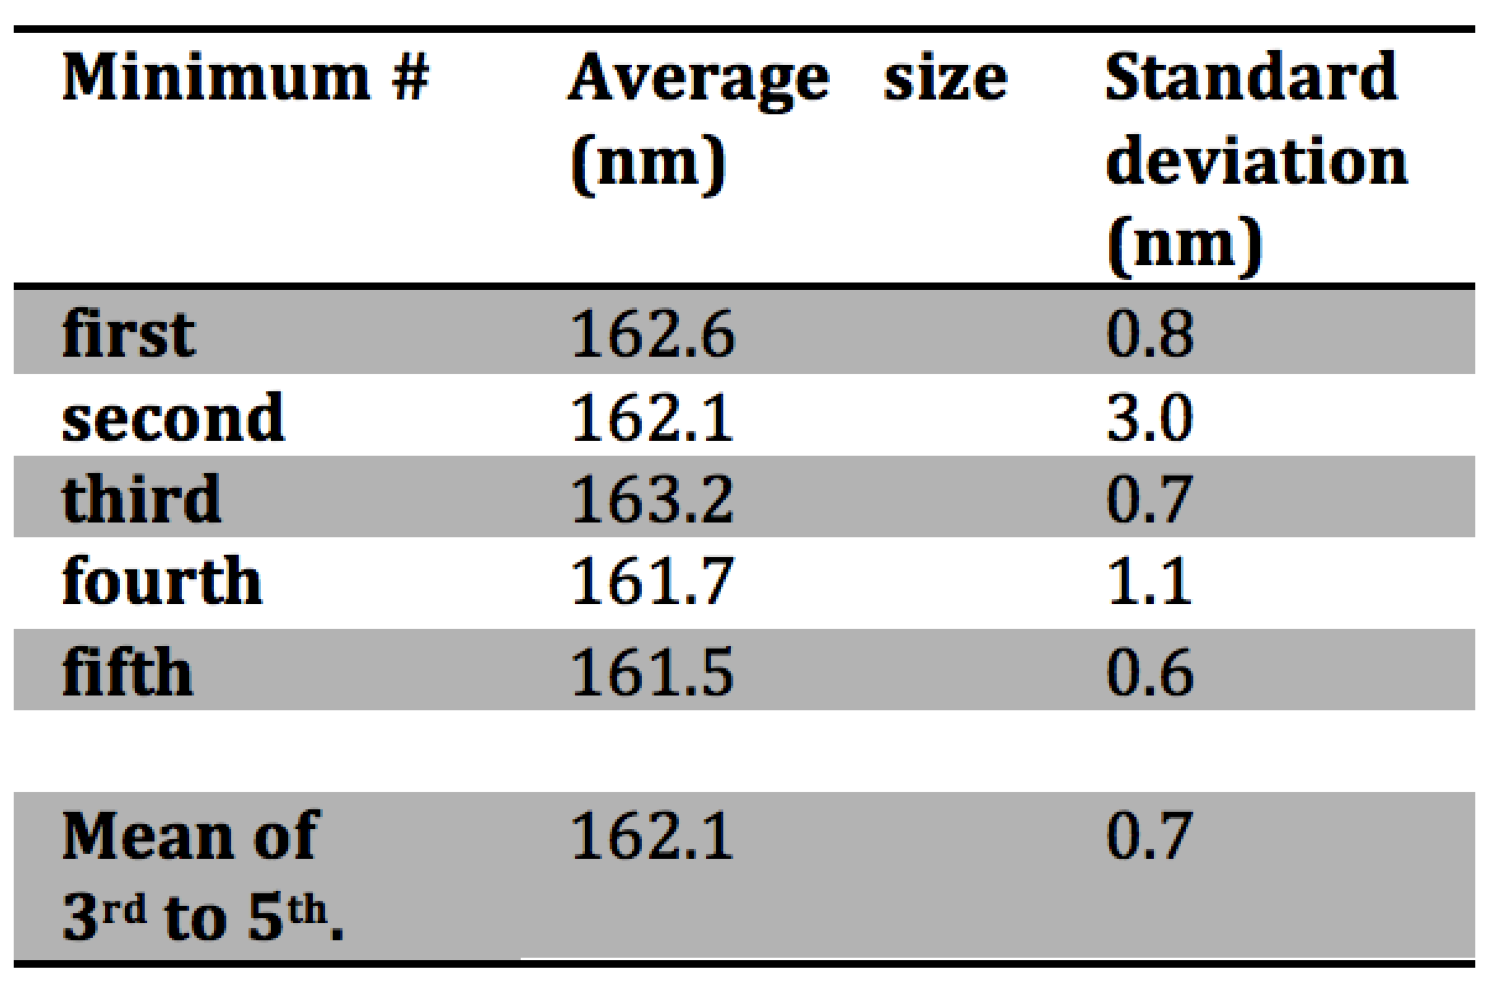
\includegraphics[width=65mm]{Chapter_08_ImageClassification_Stats.png}
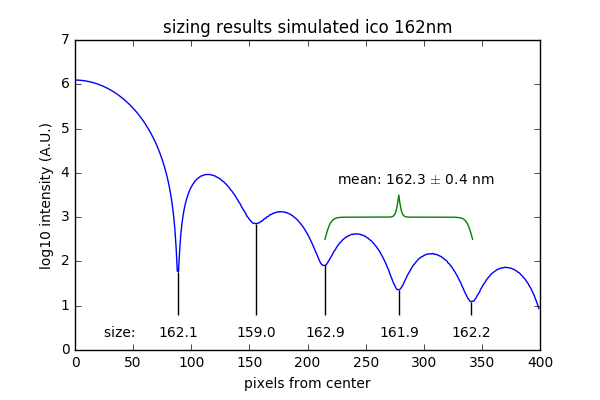
\includegraphics[width=100mm]{Chapter_08_ImageClassification_Sizing_Results.png}

\caption{Evaluation of the size assessment of a icosahedrally shaped particle of 162 nm, using the location of different minima. a) An example of the simulated diffraction patterns used in this evaluation. Each diffraction pattern has a random orientation with respect to the beam. b) The radial average of the diffraction pattern a) with associated size estimates corresponding to the location of each minima. c) the average size estimates based on the location of the each minima, and their respective standard deviations. Although the first minimum is the best in determining the size of an object by itself, the mean of the 3rd - 5th minima are also very good in determining the size of the object.}\label{fig:shape_assessment}
\end{figure}


\subsection{Edge detection}
Some objects are characterized by having sharp edges. A sharp edge in real space corresponds to a streak in the direction perpendicular to the edge in Fourier space. Objects and/or orientations of objects might be classified by determining if streaks are present, and how many. Figure explains the idea behind a streak finding algorithm.

\begin{figure}[h]
\centering
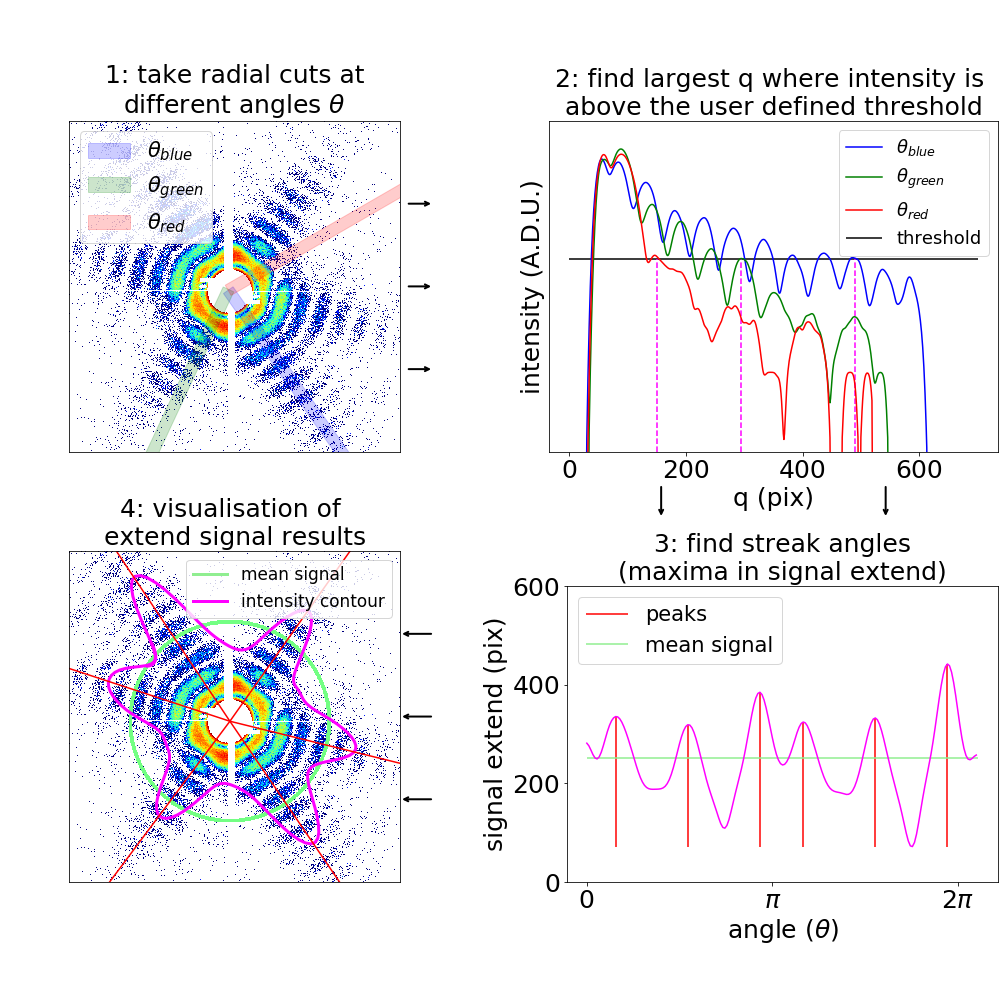
\includegraphics[width=120mm]{Chapter_08_ImageClassification_Edge_Detection.png}
\caption{An evaluation of where in the diffraction pattern the signal is located. In the first step radial cuts are taken each \textit{n} degrees. In 1) only three cuts are visualized: the blue cut is on a streak, the green one is on the edge of a streak, and the red one is in between two streaks. In step 2 the largest distance from the center where the intensity is above a user-defined thereshold is determined. These points are indicated by the dashed magenta lines in 2). The three cuts from 1) show a difference in signal extend. In step three the maxima in the signal extend are determined (see 3). If a maximum has a 180 degree pair, we consider the pair coming from a streak. The average signal extend is indicated by the lightgreen line. 4) The magenta lines contours the signal extend in the diffraction pattern. The red lines indicates the streak location and the lightgreen circle is the mean signal level.}\label{fig:edge_detection}
\end{figure}

\subsection{Elongation}

It might also be possible to determine the elongation of the particle, either by evaluating the elongation of the central speckle \cite{Hantke2014,Daurer2017} or by evaluating the elongation of the central term in a filtered autocorrelation. This is useful in discerning between diffraction from spherical and non-spherical objects. Figure \ref{fig:shape_assessment} shows two diffraction patterns: A and B. Diffraction pattern A originates from a icosahedral object and thus has a round central speckle (CS\_A). The fraction of the shortest distance from the center of the central speckle to the edge of the central speckle (minor) divided by the longest distance is called the elongation $\epsilon_{DP}$. Round central speckles have an elongation of 1. The central speckle of pattern B (CS\_B) is much more elongated. 

The evaluation of both the autocorrelations show a similar trend. AC\_A shows a roundish particle, whereas AC\_B shows a density that is more elongated. In the radial average of AC\_A and AC\_B this becomes visible as a mass beyond the maximum. The green area is considered to be part of a round particle, and the red area is considered to be part of an elongated particle. The fraction of the green area divided by the green plus the red area constitutes the elongated parameter $\epsilon_{AC}$ \footnote{Of course both these methods does not say anything about the elongation of the particle in the direction of the beam.
} The autocorrelation can only be used for the evaluation of convex objects, as non-convex object might appear roundish. 

\begin{figure}[h]
\centering
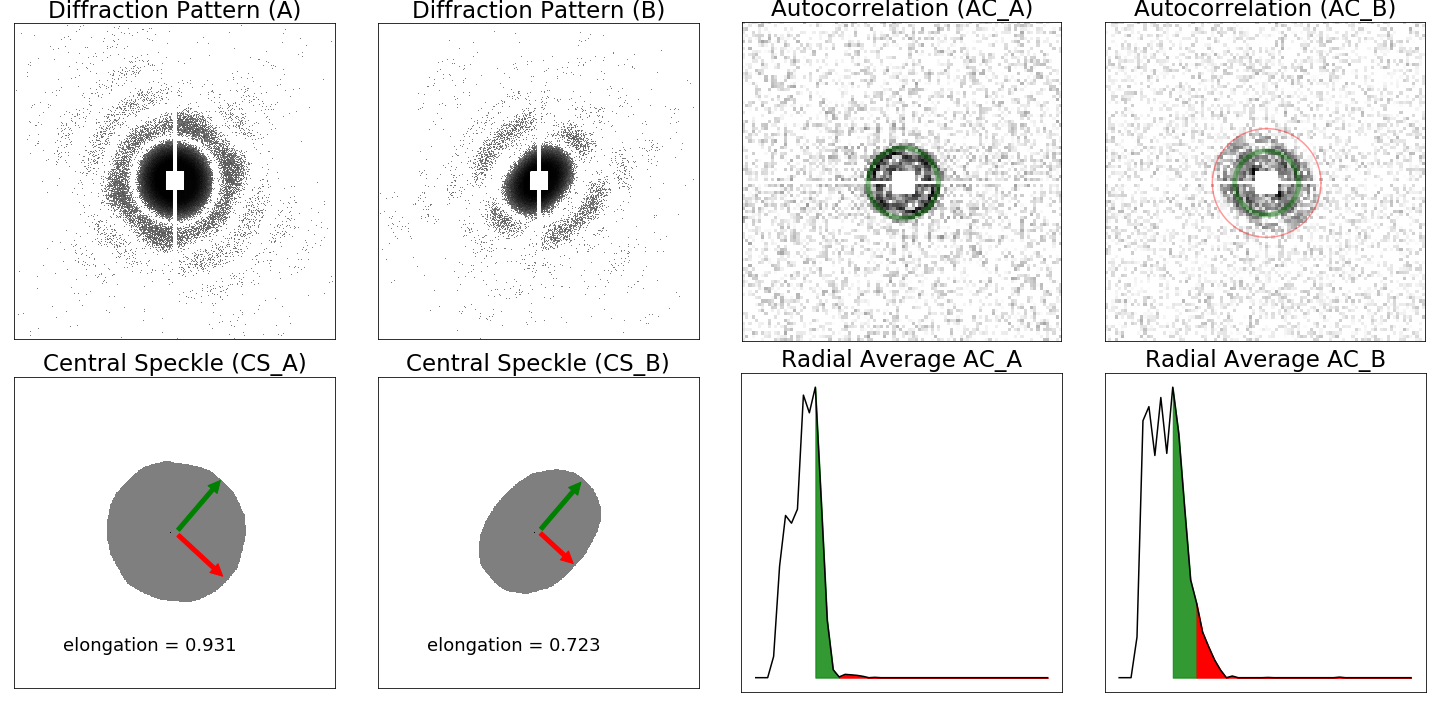
\includegraphics[width=120mm]{Chapter_08_ImageClassification_shape_assessment.png}
\caption{Elongation assessment of the particles that gave rise diffraction pattern A and B. From the central speckles of A and B, CS\_A and CS\_B, have a different shape. The elongation factor $\epsilon_{DP}$ is the fraction of the minor over the major axis of the central speckle. If $\epsilon_{DP}$ is close to 1, the objects that gace rise to the diffraction pattern is considered round in projection. The smaller $\epsilon_{DP}$ the more elongated the particle is considered. The evaluation of the autocorrelation plots show similar results. The central blob in AC\_A is roundish, whereas the central blob is more elongated in AC\_B. In the radial averages of both AC\_A and AC\_B the size of the object is taken as the maximum. The green density is considered part of a spherical object. The red density is considered part of an elongated object. $\epsilon_{AC}$ is the fraction between the green area over the green area + the red area. The closer this fraction is to 1, the more round the particle is considered.}\label{fig:shape_assessment}
\end{figure}


\subsection{The shape of the particle}
Particle shape or at least the particle size is important for automated phasing. So far automated routines have mainly dealt with icosahedral or round particles, as the size determined from the central speckle is enough to determine an accurate support constraint \cite{Hantke2014,Daurer2017}. The support size (and shape) of elongated particles such as most cells and many virus species cannot be accurately guessed in this way. This section introduces a method that can make a rough support guess for elongated particle by tracing the contour of the central term of in a filtered autocorrelation. This method uses a Lorentz based edge detection \cite{mathworks2018}.
Figure \ref{fig:detailed_shape_assessment} shows an example of how particle shape assessment using Laplace edge detection performs.

\begin{figure}[h]
\centering
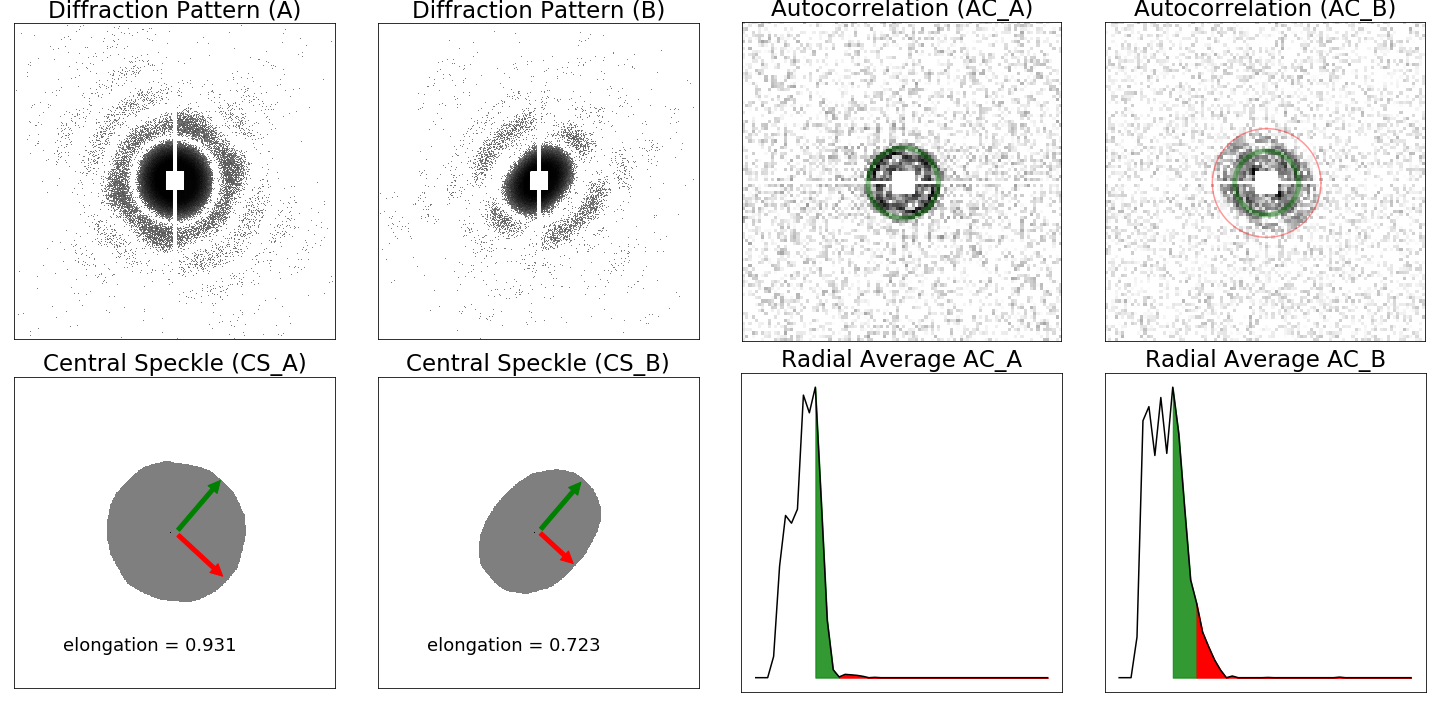
\includegraphics[width=120mm]{Chapter_08_ImageClassification_shape_assessment.png}
\caption{Finding the shape of the particle. a) shows the filtered autocorrelation of the particle. b) shows the autocorrelation after applying the laplacean edge detection. c) shows the selected area within the autocorrelation. It matches the central term of the autocorrelation. This shape can be used to determining the major and minor size of the particle, and possibly as a guess for the support or support size. }\label{fig:detailed_shape_assessment}
\end{figure}


\subsection{Multiple scatterers in the focus}

Due to the stochastic nature of the injection method, two particles can end up in the interaction region at the same time. If the particles are attached to each other, a similar pattern as seen in figure \ref{fig:shape_assessment} will occur. If the two particles are separated in space, the scattered signal of the two particles will interfere. As a result so called Newton rings will be observed in the diffraction pattern (See Figure \ref{fig:moire_pattern}. These rings code for phase information, that simply can be retrieved from the autocorrelation, as shown in Paper XX. The resolution of the reconstruction will be related to the size scatterer, the amount of missing data, and the strength of the signal. Without going into detail as to why this is the case, it can be easily understood that such patterns should be separated from the patterns originating from single particles. This section describes a method that identifies patterns coming from multiple scatterers, by identifying the presence of non central terms in the autocorrelation (these are so-called holograms). 

The first method will calculate the autocorrelation plot of the diffraction pattern, mask areas that are heavily affected by artefacts, and subtract the autocorrelation of a representative diffraction pattern. The latter is done to limit the main source of noise in the autocorrelation plot, originating from the missing data. Based on the size estimate of the particle, a central area is also masked. The error score associated with whether there are two particles present simultaneously in the focus is called $\Sigma_{HF}$. $\Sigma_{HF}$ is the median value in the autocorrelation divided by the maximum. If $\Sigma_{HF}$ is close to 1, there is most like only one particle in the beam. A threshold of 0.9 is regularly taken as the threshold for the presence of multiple particles, separated at a distance from each other.

As method one is limited in observing holograms that are located closely to the central term, a second method is needed. In this method the autocorrelation is calculated for small patches of the diffraction pattern (See Paper XIX). The advantage of selecting  patches is that their location can be chosen such that these autocorrelation plots will be less affected by possible missing data. The error metric $Sigma_{HP}$ is calculated in the same way as $\Sigma_{HF}$. The threshold for $\Sigma_{HP}$ is usually 0.3. It may however be the case that the interference structure is rather faint, such that none of the selected patches detect it. In this cases the former method for multiple selection has a higher chance to succeed.

Figure \ref{fig:Multiple_distance_assessment} shows an example of how particles are evaluated using the two methods. The left most panel shows the measured diffraction pattern. Notice the circular rings that have a center somewhere beyond the top right corner. These rings are the interference terms of the two particles. b) shows the autocorrelation of the full pattern a, after subtracting the autocorrelation of the diffraction pattern of an average particle (reference particle), and masking a central region, and a central cross. The latter also reduces artefacts. c) shows the autocorrelation of a small part of the diffraction pattern. This autocorrelation is generally less tainted by artefacts, but for weak interference signal a small region might be too small to pick up a significant signal.

\begin{figure}[h]
\centering
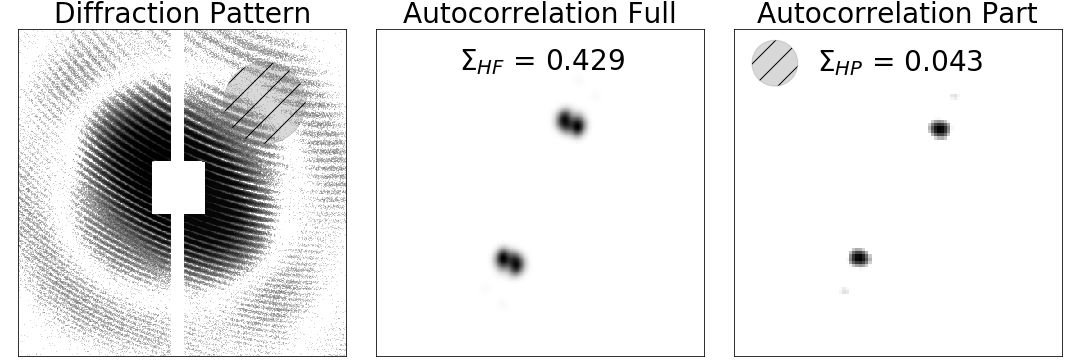
\includegraphics[width=120mm]{Chapter_08_ImageClassification_Multiple_Finding.png}
\caption{Assessing the prescence of multiple particles in the focus, located at a distance from each otherFinding the shape of the particle. a) shows a diffraction pattern which has clear circular interference rings present (center of the rings are somewhere beyond the top left corner. Note the gray circular area. This area of the diffraction pattern is used in c). b) shows the autocorrelation of a) after subtraction an average autocorrelation. The subtraction helps to reduce artefacts coming from the missing data. c) shows the autocorrelation of a small circular area in a). Both methods give two peaks.  }\label{fig:detailed_shape_assessment}
\end{figure}